\documentclass[12pt,a4paper,titlepage]{report}
\usepackage[utf8]{inputenc}
\usepackage[german,english]{babel}
\usepackage[T1]{fontenc}
\usepackage{amsmath}
\usepackage{amsfonts}
\usepackage{amssymb}
\usepackage[left=2cm,right=2cm,top=2cm,bottom=2cm]{geometry}
\usepackage[]{hyperref}
\hypersetup{
	colorlinks,
	linkcolor = blue
}
\usepackage{graphicx}
\usepackage{float}

\author{MaMaKow}
\title{Documentation \\pharmacy duty roster}

\begin{document}
\maketitle
\tableofcontents


\chapter{Introduction}
Pharmacy Duty Roster (PDR) is a web application that allows to operate a duty roster for pharmacies.
PDR started in 2015 as an alternative to a really simple excel sheet without formulas.
PDR aims to be user-friendly but at the same time cover all necessary features.
PDR continuously strives to improve. It is open to your requests and wishes.
I hope it will fulfil your expectations.
\section{Getting PDR}
The latest release of PDR is available on \href{https://github.com/MaMaKow/dienstplan-apotheke/releases/latest}{GitHub}. GitHub provides the source code as *.zip file or *.tar.gz ball. Extract the files into a folder.

Make sure to unpack PDR to a directory, that your webserver has access to. PHP and the webserver must have read access to all the files and folders. It also needs write access to the subdirectories upload, tmp and config. You might want to change the owner of the directory to the webservers user with e.g.:

You can also clone the repository with git:
\begin{verse}
git clone https://github.com/MaMaKow/dienstplan-apotheke.git
\end{verse}
See the Administrator manual for details!

\section{License}
PDR is open source software under the AGPL license.
\begin{quote}
	Copyright (C) 2018  Dr. Martin Mandelkow
	
	This program is free software: you can redistribute it and/or modify
	it under the terms of the GNU Affero General Public License as
	published by the Free Software Foundation, either version 3 of the
	License, or (at your option) any later version.
	
	This program is distributed in the hope that it will be useful,
	but WITHOUT ANY WARRANTY; without even the implied warranty of
	MERCHANTABILITY or FITNESS FOR A PARTICULAR PURPOSE.  See the
	GNU Affero General Public License for more details.
	
	You should have received a copy of the GNU Affero General Public License
	along with this program.  If not, see <https://www.gnu.org/licenses/>.
	
\end{quote}
 Please see the \href{https://github.com/MaMaKow/dienstplan-apotheke/blob/master/LICENSE.md}{license file} for details!
\section{Reporting bugs}
The issue tracker is currently located at GitHub.
GitHub requires an account in order to report bugs or feature requests. If you do not want to create one, you might send a mail to pdr-issues@martin-mandelkow.de
\section{How to contribute}
Pull requests are desired. If you made changes to PDR and want to contribute them to the public, you are welcome to open a pull-request on GitHub or send your changes in any other way.

\chapter{User manual}


\section{The web interface}
You can connect to your PDR instance using any web browser. Just navigate to your server and enter your username and password.

\subsection{Login}
\begin{figure}[h]
	\centering
	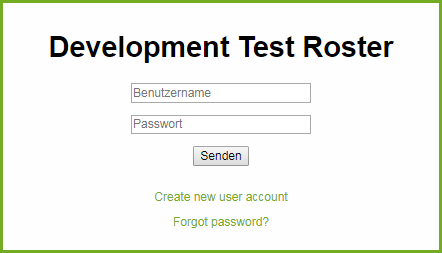
\includegraphics{{images/en_GB/login.php}.png}
	\caption{Login page}
\end{figure}
The login page shows the name of the application. You are prompted to enter your username and password.
If you do not have an account yet, you can create one. Just follow the link.
If you have an account, but forgot about your password, or want to change it, you can click on "Lost password?".

\subsection{Lost password}
\begin{figure}[h]
	\centering
	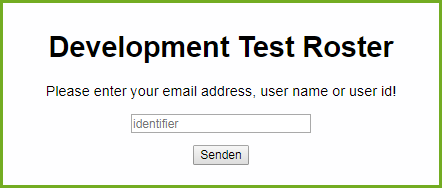
\includegraphics{{images/en_GB/lost_password.php}.png}
	\caption{Lost password page}
\end{figure}
The lost password page shows the name of the application. You are prompted to enter either your username, id or your email-address at your option.
After you submit the form, an email is sent to your stored email address.
In that email you will find a link. That link will lead you to the password change page.
\subsubsection{Lost password recovery}
\begin{figure}[h]
	\centering
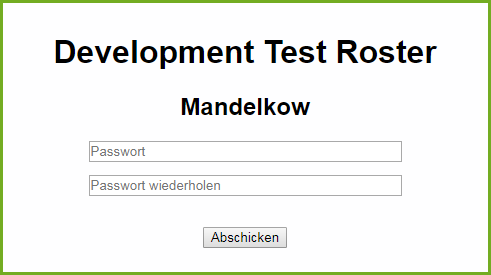
\includegraphics{{images/en_GB/reset-lost-password.php}.png}
	\caption{Lost password recovery page}
\end{figure}
The lost password recovery page shows the name of the application and your user name. You are prompted to enter a new password twice.
\subsection{Create new user account}
\begin{figure}[h]
	\centering
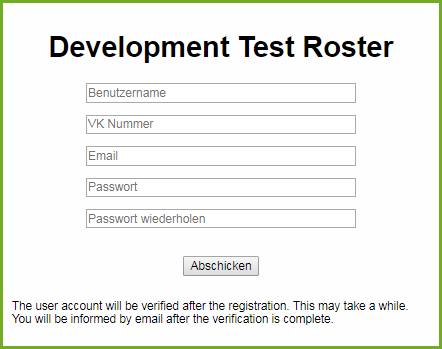
\includegraphics{{images/en_GB/register.php}.png}
	\caption{Register new user page}
\end{figure}
\subsection{Navigation}
\begin{figure}[h]
	\centering
	
\includegraphics{{images/en_GB/navigation}.png}
	\caption{Navigation bar}
\end{figure}
By default, the PDR web interface opens to your a menu containing 5 tiles.
You can navigate to:
\begin{itemize}
\item Roster week table view
\item Roster daily view
\item Roster employee view
\item Overtime 
\item Absence
\end{itemize}
\subsubsection{The navigation bar}
In the top there is a navigation bar containing hyperlinks to nearly all the pages of PDR.

\subsubsection{Roster week table view}
\subsubsection{Roster daily view}
\subsubsection{Roster employee view}
\subsubsection{Overtime}
\subsubsection{Absence}
There are four views to the absence data.
\begin{itemize}
\item Employee view readonly
\item Employee view edit
\item Monthly table
\item Year overview
\end{itemize}
In the \emph{Employee view readonly} there is a select element to choose the employee to view. There is a button to switch to the edit view.
And there is a table containing the absence data. The columns are start and end of the absence, reason of absence and number of days.
There is a distinct list of possible reasons ( vacation,
        remaining holiday,
       sickness,
        sickness of child,
        unpaid leave of absence,
        paid leave of absence,
        parental leave and
        maternity leave).
The number of days of absence is calculated for a 5 day week. Absences on saturdays and sundays are registered but not counted. The same applys for holidays.


\chapter{Administrator manual}
\section{Installation}\label{sec:installation}
\section{Upgrading}
\section{Configuration}
\section{Maintenance}
\section{Issues and Troubleshooting}


\chapter{Developer manual}
\section{Core development}
\section{Documentation}
This documentation about a programm, app or script is a stub. You can help this project by expanding it.

\section{Testing}
\section{Bug tracker}
\section{Translation}
\subsection{Internationalization}
Different counties have different laws regarding pharmacies and employment. They also have different holidays.
\end{document}
